\documentclass[11pt]{article}

\usepackage[french]{babel}
\usepackage[utf8]{inputenc}
\usepackage{fancyhdr}
\usepackage{lastpage}
\usepackage{graphicx}
\usepackage{amsmath}

%\usepackage{graphvizzz}

%\usepackage[usenames,dvipsnames]{pstricks}
%\usepackage{epsfig}
%\usepackage{pst-grad} % For gradients
%\usepackage{pst-plot} % For axes

\usepackage{enumitem}

\usepackage{framed}

%%%%%%
% Pour mise-en-forme des fichiers Ada
%
% voir exemple en fin de ce fichier.
%
% ATTENTION, requiert encoding utf-8 (voir 2ième "\lstset" ci-dessous)
 
\usepackage{listings}
%\lstset{
%  morekeywords={abort,abs,accept,access,all,and,array,at,begin,body,
%      case,constant,declare,delay,delta,digits,do,else,elsif,end,entry,
%      exception,exit,for,function,generic,goto,if,in,is,limited,loop,
%      mod,new,not,null,of,or,others,out,package,pragma,private,
%      procedure,raise,range,record,rem,renames,return,reverse,select,
%      separate,subtype,task,terminate,then,type,use,when,while,with,
%      xor,abstract,aliased,protected,requeue,tagged,until,printf},
%  sensitive=f,
%  morecomment=[l]--,
%  morestring=[d]",
%  showstringspaces=false,
%  basicstyle=\tiny\ttfamily,
%  keywordstyle=\bf\tiny,
%  commentstyle=\itshape\tiny,
%  stringstyle=\sf\tiny,
%  extendedchars=true,
%  columns=[c]fixed
%}
\usepackage{color}
\definecolor{mygreen}{rgb}{0,0.6,0}
\definecolor{mygray}{rgb}{0.5,0.5,0.5}
\definecolor{mymauve}{rgb}{0.58,0,0.82}
\definecolor{myblue}{rgb}{0,0,0.82}

\lstset{%
  morekeywords={abort,abs,accept,access,all,and,array,at,begin,body,
      case,constant,declare,delay,delta,digits,do,else,elsif,end,entry,
      exception,exit,for,function,generic,goto,if,in,is,limited,loop,
      mod,new,not,null,of,or,others,out,package,pragma,private,
      procedure,raise,range,record,rem,renames,return,reverse,select,
      separate,subtype,task,terminate,then,type,use,when,while,with,
      xor,abstract,aliased,protected,requeue,tagged,until,printf},
  basicstyle=\scriptsize\ttfamily,%
  commentstyle=\color{mygreen}\footnotesize\ttfamily,%
  frameround=trBL,
  frame=single,
  breaklines=true,
  showstringspaces=false,
  numbers=left,
  numberstyle=\tiny,
  numbersep=10pt,
  language=Java,
  morekeywords={Math},
  keywordstyle=\color{myblue}\bf
}

% CI-DESSOUS: conversion des caractères accentués UTF-8 
% en caractères TeX dans les listings...
\lstset{
  literate=%
  {À}{{\`A}}1 {Â}{{\^A}}1 {Ç}{{\c{C}}}1%
  {à}{{\`a}}1 {â}{{\^a}}1 {ç}{{\c{c}}}1%
  {É}{{\'E}}1 {È}{{\`E}}1 {Ê}{{\^E}}1 {Ë}{{\"E}}1% 
  {é}{{\'e}}1 {è}{{\`e}}1 {ê}{{\^e}}1 {ë}{{\"e}}1%
  {Ï}{{\"I}}1 {Î}{{\^I}}1 {Ô}{{\^O}}1%
  {ï}{{\"i}}1 {î}{{\^i}}1 {ô}{{\^o}}1%
  {Ù}{{\`U}}1 {Û}{{\^U}}1 {Ü}{{\"U}}1%
  {ù}{{\`u}}1 {û}{{\^u}}1 {ü}{{\"u}}1%
}

%%%%%%%%%%
% TAILLE DES PAGES (A4 serré)

\setlength{\parindent}{20pt}
\setlength{\parskip}{1ex}
\setlength{\textwidth}{17cm}
%\setlength{\textwidth}{16cm}
\setlength{\textheight}{23cm}
\setlength{\oddsidemargin}{-.7cm}
\setlength{\evensidemargin}{-.7cm}
\setlength{\topmargin}{-.5in}

%%%%%%%%%%
% EN-TÊTES ET PIED DE PAGES

\pagestyle{fancyplain}
\renewcommand{\headrulewidth}{0pt}
\addtolength{\headheight}{1.6pt}
\addtolength{\headheight}{2.6pt}
\lfoot{}
\cfoot{}


%%%%%%%%%%
% titre du document

\title{Algorithms \\
	\textbf{``Hold'em for n00bs''}}

\author{Thanh Luan, Six Cyril, Vial Loïc \\
			Rouby Thomas, Marriott Richard\\
			Poupin Pierre} 

\date{7\up{th} of November 2014}


\begin{document}

\maketitle

\section{Introduction}
The game we are playing is quite simple : It is a turn based two-player game, using a line of cards : Each player can take either the left-most card or the right-most card.
The winner is the one who gets the highest value calculated by the sum of cards.
We assume that we play with a basic artificial intelligence, which always pick the highest valued card.

We will present several types of algorithms to win in most cases : a greedy one, a full-exploration one, and a dynamic one.

The greedy algorithm is simply what the IA does, we hope to win at the end, but we are not sure if we will succeed, whereas the full-exploration of space's method checks every combination of cards' picking, to find a solution in advance, and then we can apply it.
The dynamic programming algorithm is basically optimizations we made on the full exploration algorithm, to enhance the performances and lessen the costs in memory and time.

We will now present with more details those algorithms.


\section{The greedy algorithm}
\subsection{What is a greedy algorithm?}

A greedy algorithm is one that attempts to make the best decision it can based on a small amount of immediately available information..........

(talk about selecting the maximum card, exemplified below.)

\subsection{Implementation of the game using a greedy algorithm}
Let's take a deeper look at the game and his basic algorithm :
To prepare the game, we have to shuffle the cards, and display them in a one-dimension array.
Then, we have to design two strategies : ours, and the one that the computer/IA/sister will use : The last one simply chooses the highest valued card between the two availables.
Our strategy will be the algorithms we talked previously in the introduction.
Finally, the game consists only in the alternance of the two strategies of the player.
To simulate the fact that we pick a card, we use two indexes that represents the limits of the array of cards : Upon picking a card, we increment (decrement) the left (right) index if we chose the left (right) card. The game is finished when the last card is picked, that is to say when the indexes are equal.

\subsection{Implementation}
\begin{lstlisting}
int cards[52];

shuffle_deck()
	for i = 1 to 4
		for j = 1 to 13
			cards[(i-1)*13+j] = j + 1
	// Now shuffle cards
	for i = 1 to 52
		one = rand(0,51)
		two = rand(0,51)

		temp = cards[one]
		cards[one] = cards[two] // Swap cards at two randoom positions
		cards[two] = temp

int sister(int left, int right)
	if cards[left] > cards[right]
		return left
	
	return right


int strategy (int left, int right)
	if cards[left] > cards[right]
		return left

	return right


void play_game ()
	int left = 0
	int right = 51
	int my_total = 0
	int sis_total = 0
	bool my_turn = true

	while (left != right)
		if my_turn
			choice = strategy(left,right)
			my_total = my_total + cards[choice]
		else
			choice = sister(left,right)
			sis_total = sis_total + cards[choice]

		if choice == left
			left++
		else
			right--

		my_turn = !my_turn

	// Final Card
	if my_turn
		my_total = my_total + cards[left]
	else
		sis_total = sis_total + cards[left]
\end{lstlisting}

\subsection{Assessment of the greedy algorithm}

The sister's version of the greedy algorithm is very simple to implement - only requiring three of four lines of code - and is very cheap to execute, the decision being based on only a single comparison of cards. However, as both the primary player and the sister are employing the same strategy, the player that wins the game is essentially left to chance.

An alternative (fairly) greedy strategy is to only select the highest card if it does not reveal a higher card to the sister............

\section{Full solution-space algorithm}
\subsection{Explanation}
This algorithm explores every sequences of possible decisions. Each decision can
be either "take the right card" or "take the left card", so a decision can be
represented by a boolean.

Thus, a sequence of decisions is a sequence of booleans ; and to each sequence 
of booleans an integer can be associated : for example, if we have the sequence
$(b_n)$, we associate the binary number $b_nb_{n-1}..b_0$.

As a consequence, a strategy is represented by an integer ; and
exploring each possible strategies is done by iterating from strategy 0 to the
strategy $2^{\lceil{N/2}\rceil} - 1$, and keeping the best one.

To decide whether the sister starts or not, both cases are computed, and
the one that grants the highest score is kept.

In this algorithm, in order to avoid recomputing already-computed values,
a tree is built along each iteration. Each node represents a step in the game,
and contains : a list of remaining cards and the score obtained so far.

Below (figure \ref{tree}) is an example of a tree drawn 
for the list of cards $[5, 2, 6]$.
\begin{figure}[ht]
	\center
	\label{tree}
	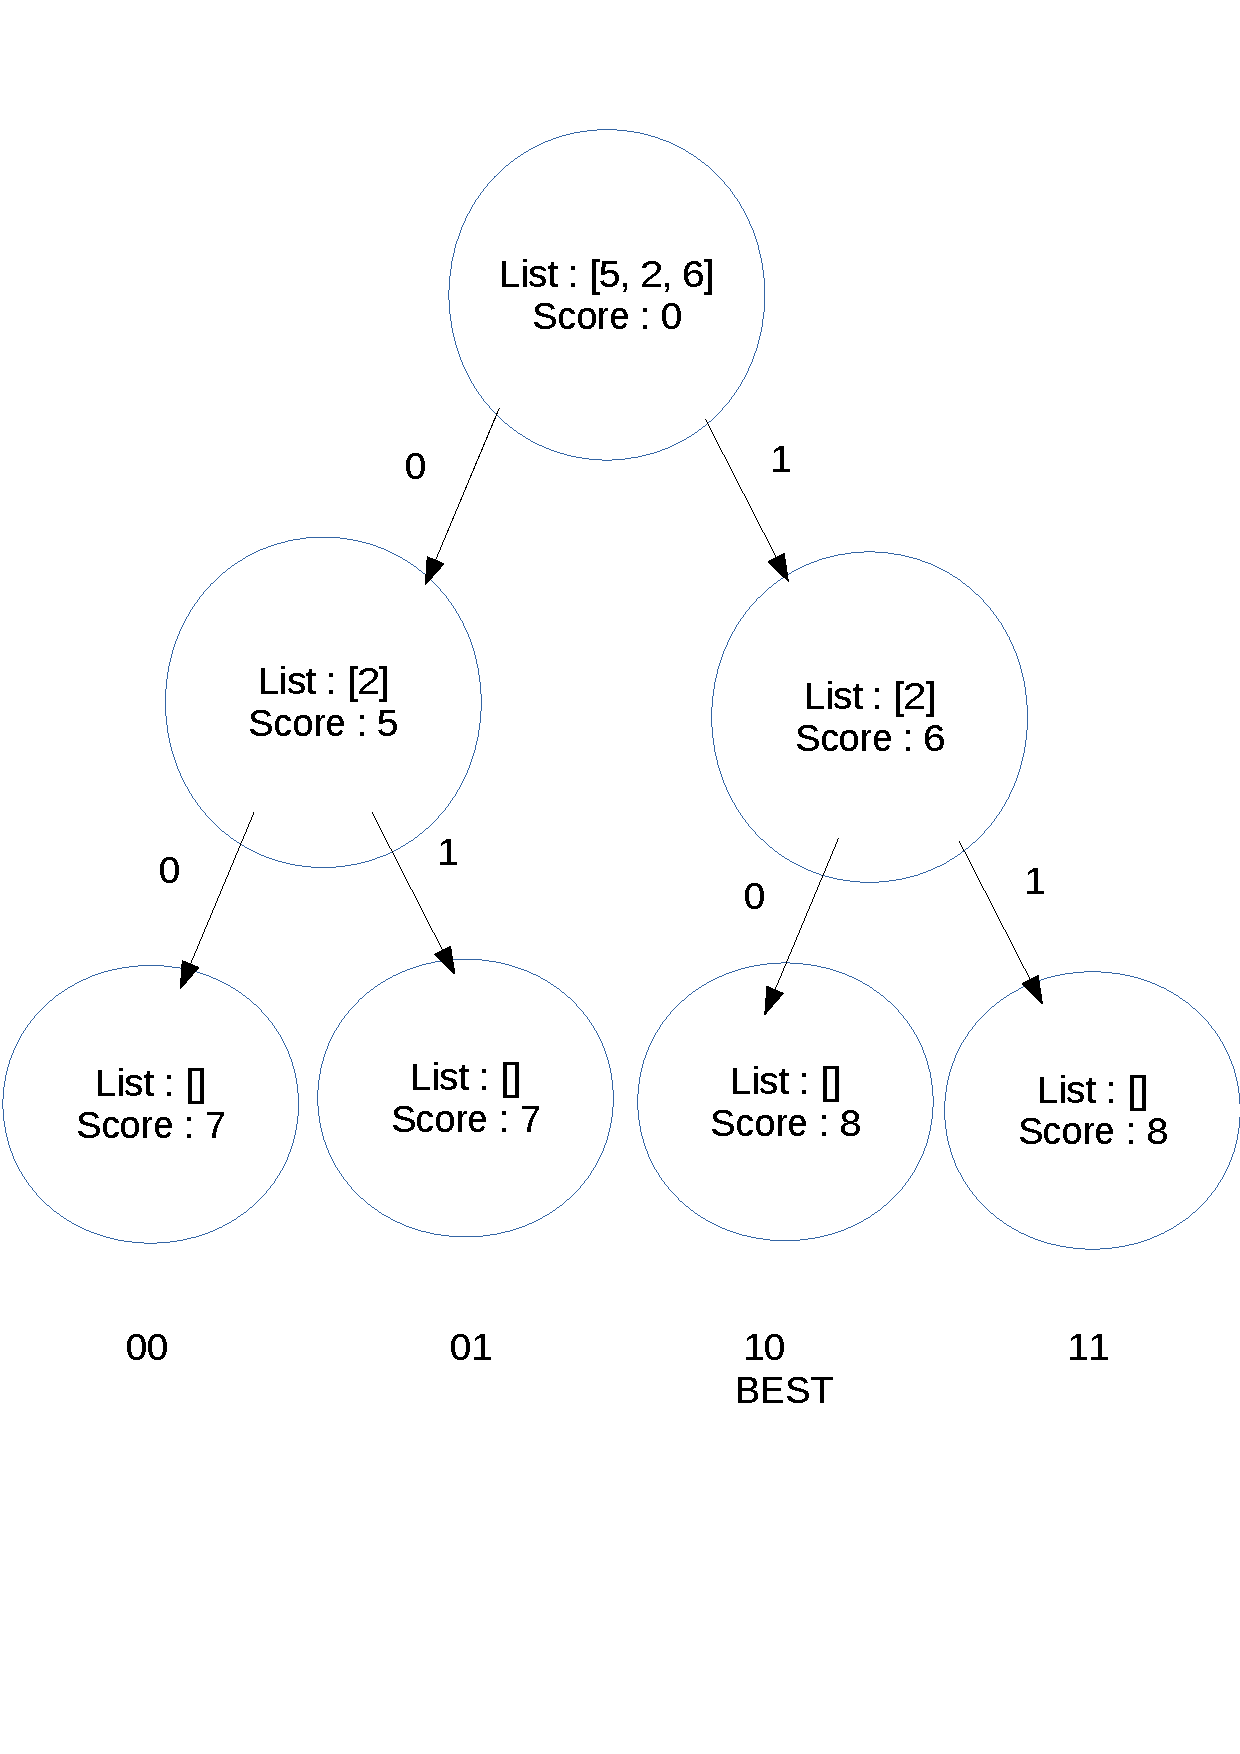
\includegraphics[width=0.32\linewidth]{complete_space.pdf}
	\caption{Tree of all possible decisions for [5, 2, 6]}
\end{figure}

\subsection{Algorithm}
\begin{lstlisting}
/**
 * Side note : for the implementation, instead of storing the entire lists in
 * every nodes, we can just store the value of starting and finishing indexes
 * For example, instead of having [L[3], L[4], L[5]] we can just store 3 and 5
 * in the node
 */
struct Node is :
|	List L // list of remaining card values
|	int val // the current score when we reach the node
|	Node *node[2] // the sons, enum{LEFT=0, RIGHT=1}
end

/* Returns the best decision, and the value obtained with this decision */
best_strategy(L) return (int, int) is :
|	N = len(L)
|	
|	start = new Node(L, 0, NULL, NULL)
|	best_val = -1
|
|	for decision from 0 to 2^(ceil(N/2)) - 1 do:
|	|	current = start
|	|	for i from N-1 to 0 by -1 do:
|	|	|	cur_L = current->L
|	|	|	cur_N = len(cur_L)
|	|	|	cur_val = current->val
|	|	|	take_right = (decision >> i) // shifted
|	|	|	
|	|	|	if (current->node[take_right] == NULL):
|	|	|	|	if take_right:
|	|	|	|	|	new_L = L \ L[cur_N - 1] \ max(L[0], L[cur_N - 2])
|	|	|	|	|	new_val = cur_val + L[cur_N - 1]
|	|	|	|	else:
|	|	|	|	|	new_L = L \ L[0] \ max(L[1], L[cur_N - 1])
|	|	|	|	|	new_val = cur_val + L[0]
|	|	|	|	current->node[take_right] = new Node(new_L, new_val, NULL, NULL)
|	|	|	end
|	|	|
|	|	|	current = current->node[take_right]
|	|	done
|	|
|	|	decision_val = current->val
|	|	if decision_val > best_val:
|	|	|	best_val = decision_val
|	|	|	best_decision = decision
|	|	end
|	done
|
|	free_rec(start)
|	return (best_val, best_decision)
end

free_rec(node) is:
|	for i in {LEFT, RIGHT} do:
|	|	if node->node[i] != NULL:
|	|	|	free_rec(node->node[i])
|	|	fi
|	done
|	free(node)
end

main is :
|	L = list of card values
|	N = len(L)
|
|	val_i_start, strategy_i_start = best_strategy(L)
|	L_she_starts = L \ (max(L[0], L[N-1]))
|	val_she_starts, strategy_she_starts = best_strategy(L_she_starts)
|
|	if val_i_start >= val_she_starts:
|	|	echo "The best strategy is $strategy_i_start, and i have to start"
|	else:
|	|	echo "The best strategy is $strategy_she_starts, and she has to start"
|	end
end

\end{lstlisting}

\subsection{Complexity}
In the end, $2^{\lceil{N/2}\rceil} - 1$ decisions have been computed, which
requires $2^{\lceil{N/2}\rceil+1} - 1$ nodes to be created.

If we consider that the access times are negligeable, then we have a
complexity of $O(2^{N/2})$ : both in terms of memory and time, the
complexity is exponential.

We can get rid of the exponential complexity for the memory if we delete
nodes that we do not need anymore along the creation of the tree (keeping only
the current and best branches, that would make a memory complexity of $O(N)$), 
but the exponential complexity for computation time remains.
\section{Dynamic implementation}
Starting with a full pack of cards, unless the final two cards are the left-most pair or the right-most pair, there is always more than one sequence of card selections that will lead to us having that final remaining pair. The recursive formula above therefore describes the problem as a ``linked tree'' (i.e. a triangular lattice where where the right and the left children of any two horizontally adjacent nodes are the same node) of subproblems where each subproblem is not unique. We argue that this recursive function will calculate the optimal score when provided with the appropriate base cases.


\footnotesize
\begin{align*}
	Best(i, j) = Max\left( 
	\left[C[i] +
	\begin{cases}
		Best(i+2,j) & \text{if $C[i+1] > C[j]$} \\
		Best(i+1,j-1) & \text{otherwise}
	\end{cases}
	\right]
	,
	\left[
	C[j] +
	\begin{cases}
		Best(i+1,j-1) & \text{if $C[i] > C[j-1]$} \\
		Best(i,j-2) & \text{otherwise}
	\end{cases}
\right]
	\right)
\end{align*}
\normalsize

\subsubsection*{Example}
	$\text{Cards } = \{5,7,9,1,4,2\}$

	\begin{tabular}[c]{cc|cccccc}
		& $i$ $\rightarrow$\\

		$j$          &   & 1 & 2 & 3 & 4 & 5 & 6 \\
		             \cline{2-8}
		$\downarrow$ & 1 & 5 & X & X & X & X & X \\
		             & 2 & 7 & 7 & X & X & X & X \\
		             & 3 &   & 9 & 9 & X & X & X \\
		             & 4 &   &   & 9 & 1 & X & X \\
		             & 5 & ? &   &   & 4 & 4 & X \\
		             & 6 & ? & ? &   &   & 4 & 2
		
	\end{tabular}

\subsection{Top-down}

\subsection{Bottom-up}
As each subproblem is not unique, a recursive algorithm is at risk of performing the same calculations multiple times. The recursive, top-down version of the solution described in this paper performs a check before calculating the values for a node to ensure they haven't been calculated before. In the bottom-up version of the solution, described here, we instead start with the base cases (along the primary diagonal and the adjacent diagonal of the array pictured above) and then cycle through each of the remaining cells only a single time.

From the recursive formula you can see that $Best(i, j)$ is always dependent on a cell two steps away, towards the top-right of the pictured
array: either $(i+2), (j-2)$ or $(i+1, j-1)$. i.e. To calculate the value of ``Best'' for any cell, the next diagonal is skipped and the 
dependencies are found in the following diagonal. If we were to assume that the primary player always goes first then these diagonals 
(corresponding to the problems with which the second player is faced) would not need to be calculated - 
they could be left blank. However, the optimal solution for a player does not necessarily require them to go first. It is 
then necessary to treat them as a game with one less card, where the second player has already taken one of the cards. 
In this case, the primary player is always left with a subproblem with an odd number of cards. He/she will then 
be left with the final card - the base case along the main diagonal. If the primary player goes first then he will always 
be left with the final two cards, of which he/she would want to take the largest. The base case for the 
second diagonal is therefore $Best(i-1, i) = MAX(cards[i-1], cards[i])$.

\subsubsection*{Algorithm Details}
\begin{itemize}
		\item The structure used for the nodes (the ``problem'' structure) contains the value of ``best'' as well as a pointer to the node that is the optimal ``subproblem'', therefore forming a linked list of optimal decisions.
		\item Despite the problem being a triangular array of nodes, for simplicity we represent is as a square 2D array. As this is just an array of pointers to ``problem'' structures, it wouldn't take up as much space as it could.
		\item Once the values of the nodes of the array have been calculated, the optimal scores for the cases where you go 
			first and when your sister goes first (and selects the maximum initial card) are compared. The global boolean variable, 	
			LET\_SISTER\_GO\_FIRST, is then set and the winning node returned by the function.
\end{itemize}

\subsection{Implementation}
\begin{lstlisting}
struct problem
| int best // The best possible score for each problem
| problem *subproblem // Used to create a linked-list of the optimal choices

int cards[numcards] = {...}
bool LET_SISTER_GO_FIRST

problem *solve()
| problem *table[numcards][numcards] // half wasted but it's only pointers
|
| // Do base cases (Case 0 is done separately as the
| // other base cases are in done pairs)
| table[0][0] = new(problem)
| table[0][0].best = cards[0]
| table[0][0].subproblem = NULL
|
| for (i = 1; i < numcards; i++)
| | table[i][i] = new(problem)
| | table[i][i].best = cards[i]
| | table[i][i].subproblem = NULL
| |
| | table[i-1][i] = new(problem)
| | table[i-1][i].subproblem = NULL
| |
| | // In the second base diagonal, "best" should be set to the
| | // maximum value of the two cards represented by that cell.
| | if (cards[i-1] > card[i])
| | | table[i-1][i].best = cards[i-1]
| | else
| | | table[i-1][i].best = cards[i]
| 
| // Now solve the rest of the table by scanning through its diagonals
| // (thus ensuring each cell's dependencies have already been calculated)
| for (j = 2; j < numcards; j++)
| | for (i = 0; i < numcards-j; i++)
| | | table[i][i+j] = new(problem)
| | |
| | | // I choose left, sis chooses left
| | | if (cards[i+1] > cards[i+j]
| | | | left_best = cards[i] + table[i+2][i+j].best
| | | | left_sub = &table[i+2][i+j]
| | | else
| | | | // I choose left, sis chooses right
| | | | left_best = cards[j] + table[i+1][i+j-1].best
| | | | left_sub = &table[i+1][i+j-1]
| | |
| | | // I choose right, sis chooses left
| | | if (cards[i] > cards[i+j-1]
| | | | right_best = cards[i+j] + table[i+1][i+j-1].best
| | | | right_sub = &table[i+1][i+j-1]
| | | else
| | | | // I choose right, sis chooses right
| | | | right_best = cards[i+j] + table[i][i+j-2].best
| | | | right_sub = &table[i][i+j-2]
| | |
| | | // We have now found the two possible outcomes (taking
| | | // account of the sister's move), but which is best?
| | | // Set table[i][i+j] accordingly...
| | | if (left_best > right_best)
| | | | table[i][i+j].best = left_best
| | | | table[i][i+j].subproblem = left_sub
| | | else
| | | | table[i][i+j].best = right_best

| | | | table[i][i+j].subproblem = right_sub
|
| // We want to know, for this deck of cards, whether it is optimal
| // to allow your sister to have the first move or not.
| // (Both situations have been calculated.)
| if (cards[0] > cards[numcards - 1])
| | if (table[1][numcards - 1].best > table[0][numcards - 1].best)
| | | LET_SISTER_GO_FIRST = TRUE
| | | return table[1][numcards - 1]
| else
| | if (table[0][50] > table[0][numcards - 1])
| | | LET_SISTER_GO_FIRST = TRUE
| | | return table[0][50]
|
| LET_SISTER_GO_FIRST = FALSE
| return table[0][numcards - 1]
\end{lstlisting}

\section{Conclusion}

We have seen that there is more than one strategy that can be applied in order to beat your greedy sister at this simple game of cards. However, there is only one optimal strategy. It was observed that matching the sister's greedy strategy of selecting the highest available card would only lead to a victory in about 50\% of cases. While this is not an ideal result, the simple strategy benefits from being very simple to implement and being very cheap to execute, in terms of system resources; and at least it wouldn't lead to a net loss of money and of pride.

There are other greedy strategies that could be implemented - for example, only selecting the highest card if does not reveal a higher one. However, it cannot be guaranteed that such a strategy will always result in a win. One sure way to win the game is to play optimally, i.e. to make the decisions necessary to achieve the highest score possible given that particular configuration of cards, and given the opponent's strategy. To discover this optimal sequence of decisions, the entire solution-space must be explored, returning the path through it resulting in the highest score.

The initial algorithm presented here, that explores the entire solution-space, is an iterative one.\\
*** Cyril - can you explain your algorithm here?? ***\\
We identified that this algorithm was of complexity $O(n^3)$.

In an attempt to reduce the complexity of the initial full-solution-space algorithm, dynamic programming techniques were employed. i.e. we assumed that the optimal solution could be represented as the optimal solution to the current problem given that all sub-problems had been solved optimally. This lead to the recursive "Best" function given in section 4, which represents the solution space as a "triangular lattice" rather than a binary tree. A naive implementation of the "Best" function would also lead to an algorithm of complexity $O(n^3)$. However, the fact that the graph of nodes is now represented as a lattice of shared sub-problems, rather than a tree, reveals the fact that optimisations can easily be made. Rather than allowing the algorithm to visit each node multiple times, a "cache" of visited nodes was added so that calculations for already visited nodes would noit have to be re-performed. This optimisation lead to a more complicated-looking but more efficient algorithm of complexity $O(n^2)$.



%	\digraph a {
%		size="3.5,3.5";
%		a->b;
%		a->c;
%		b->d;
%		b->e;
%		c->h;
%		c->i;
%		d->k;
%		e->k;
%		h->l;
%		i->l;
%		l->m;
%		k->m;
%	}
\end{document}
